\chapter{Experiments and Results}
\label{ch:results}

This chapter presents comprehensive experimental results comparing eight INR architectures on 3D occupancy reconstruction using the Nefertiti bust mesh. We analyze quantitative metrics, examine the relationship between architectural properties and performance, evaluate computational efficiency, and characterize failure modes.

\section{Experimental Setup}
\label{sec:setup}

Our experiments evaluate all eight INR methods on the Nefertiti bust mesh, a high-resolution cultural heritage scan featuring smooth facial geometry, fine ornamental details on the crown, and sharp geometric transitions between the face and headdress. This mesh provides a challenging test for fine detail reconstruction while remaining computationally tractable for systematic comparison.

The mesh is normalized to $[-1, 1]^3$ and sampled once, ahead of training, into a fixed dataset of 500,000 labelled points: half drawn uniformly from the bounding box and half drawn near the surface with Gaussian displacement of standard deviation $\sigma = 0.01$. This gives the network training signal near boundaries, where classification is most difficult, while also teaching the global occupancy structure. Because the dataset is fixed rather than resampled each epoch, the same points are revisited throughout training.

All models share the same depth and width: 3-dimensional input $(x, y, z)$, 4 hidden layers with 256 features each, and 1-dimensional output. Matching depth and width does not match capacity, however: parameter counts range from 133{,}250 (FR) to 1{,}057{,}282 (WIRE), with most methods near 265{,}000. We return to this confound when interpreting the results. Training proceeds for 500 epochs with batch size 16,384 and initial learning rate $1 \times 10^{-4}$ following cosine annealing to $1 \times 10^{-6}$. Two methods required learning rate overrides for stable convergence: GAUSS used $1 \times 10^{-3}$ and MFN used $3 \times 10^{-4}$. Binary Cross-Entropy loss is used throughout, with gradient clipping at maximum norm 1.0.

The dataset is split into 450,000 training points and 50,000 validation points by a seeded generator, so every method is evaluated on the same held-out points. Evaluation IoU is computed on that held-out split; Chamfer-L1 and normal consistency are computed from a mesh extracted by Marching Cubes on a dense $256^3$ grid (16,777,216 points). All experiments were conducted on a single NVIDIA Tesla T4 GPU using PyTorch 2.0 with CUDA 11.8.

\section{Quantitative Results on Nefertiti Bust}

Table~\ref{tab:nefertiti_results} presents the evaluation metrics for all eight methods on the Nefertiti bust. Evaluation IoU is measured on the held-out validation split at classification threshold $\tau = 0.5$; the surface metrics are measured on the $256^3$ marching-cubes reconstruction.

% Tables are generated from results_3d_comparison.csv by make_tables.py.
% Do not edit them by hand; re-run the script after any new benchmark run.
% AUTO-GENERATED by make_tables.py -- do not edit by hand.
% Regenerate with: python make_tables.py

\begin{table}[htbp]
\centering
\caption{Quantitative results for 3D occupancy reconstruction on the Nefertiti bust (500 epochs). Evaluation IoU is measured on the held-out 50{,}000-point validation split; Chamfer-L1 and normal consistency are computed against the ground-truth mesh from a $256^3$ marching-cubes extraction. Best results in bold.}
\label{tab:nefertiti_results}
\begin{tabular}{lccccl}
\toprule
\textbf{Method} & \textbf{Eval IoU} $\uparrow$ & \textbf{Train IoU} & \textbf{Chamfer-L1} $\downarrow$ & \textbf{Normal Cons.} $\uparrow$ & \textbf{Config} \\
\midrule
INCODE & \textbf{0.9641} & 0.9725 & 0.010955 & 0.9802 & scale: 50.0 \\
Fourier Features & 0.9632 & 0.9892 & 0.010973 & \textbf{0.9809} & gamma: 256, sigma: 1.0 \\
FR & 0.9606 & 0.9976 & 0.010928 & 0.9784 & F: 64 \\
SIREN & 0.9564 & 1.0000 & 0.010905 & 0.9799 & first\_omega\_0: 30.0, hidden\_omega\_0: 30.0 \\
FINER & 0.9541 & 0.9628 & 0.010946 & 0.9789 & frequency\_bands: 16 \\
WIRE & 0.9521 & 1.0000 & \textbf{0.010903} & 0.9807 & first\_omega\_0: 40.0, hidden\_omega\_0: 20.0, sigma0: 3.0 \\
MFN & 0.9325 & 0.9385 & 0.011035 & 0.9775 & input\_scale: 10.0, alpha: 6.0, beta: 1.0 \\
GAUSS & 0.9158 & 0.9126 & 0.011190 & 0.9752 & input\_scale: 20.0, sigma: 1.0 \\
\bottomrule
\end{tabular}
\end{table}

\begin{table}[htbp]
\centering
\caption{Training time and quality-efficiency trade-off, ordered by wall-clock time. IoU/minute is evaluation IoU divided by training time in minutes.}
\label{tab:training_time}
\begin{tabular}{lccc}
\toprule
\textbf{Method} & \textbf{Time (s)} $\downarrow$ & \textbf{Eval IoU} $\uparrow$ & \textbf{IoU/minute} $\uparrow$ \\
\midrule
SIREN & \textbf{2635.3} & 0.9564 & \textbf{0.0218} \\
FR & 2680.1 & 0.9606 & 0.0215 \\
FINER & 2699.2 & 0.9541 & 0.0212 \\
Fourier Features & 2725.4 & 0.9632 & 0.0212 \\
GAUSS & 2778.2 & 0.9158 & 0.0198 \\
INCODE & 2797.1 & 0.9641 & 0.0207 \\
MFN & 2896.1 & 0.9325 & 0.0193 \\
WIRE & 3926.6 & 0.9521 & 0.0145 \\
\bottomrule
\end{tabular}
\end{table}


INCODE achieves the highest evaluation IoU (0.9641), with Fourier Features effectively tied at 0.9632 and FR close behind at 0.9606. The margin across the leading group is small: six of the eight methods fall within 1.2 percentage points of each other (0.9521--0.9641), and the top two are separated by 0.0009. Given that each configuration was run exactly once, with unseeded weight initialization and batch shuffling, we cannot claim that this ordering is meaningful. What the data supports is a separation into a leading group of six methods and a trailing pair, not a ranking within the leading group.

The two trailing methods are clearly separated. MFN reaches 0.9325 and GAUSS 0.9158, between 3.2 and 4.8 points below the leaders --- a gap large enough to survive the uncertainty that makes the leading group indistinguishable.

The surface metrics broadly agree with the IoU ordering. WIRE and SIREN achieve the best Chamfer-L1 (0.010903 and 0.010905) and GAUSS the worst (0.011190), while Fourier Features attains the best normal consistency (0.9809). The spread across all eight methods is only 2.6\% of the Chamfer value, however, and because the surface samples underlying both metrics are drawn without a fixed seed, we do not read anything into differences at the fourth decimal place.

The Fourier Features result reported here uses a frequency scale of $\sigma = 1.0$. An earlier run of the same architecture, differing only in this one hyperparameter ($\sigma = 10.0$), reached an evaluation IoU of 0.7966. We retain that run as a deliberate ablation rather than discarding it, and analyse it in Section~\ref{sec:fourier_ablation}, because the contrast between the two isolates the effect of frequency scale more cleanly than any comparison across architectures.

\section{Qualitative Results}

Figure~\ref{fig:reconstruction_comparison} compares the ground-truth bust with the strongest method (INCODE) and the weakest (GAUSS). Images are rendered at consistent viewpoint and lighting for fair comparison.

\begin{figure}[htbp]
\centering
\begin{subfigure}[b]{0.48\textwidth}
\centering
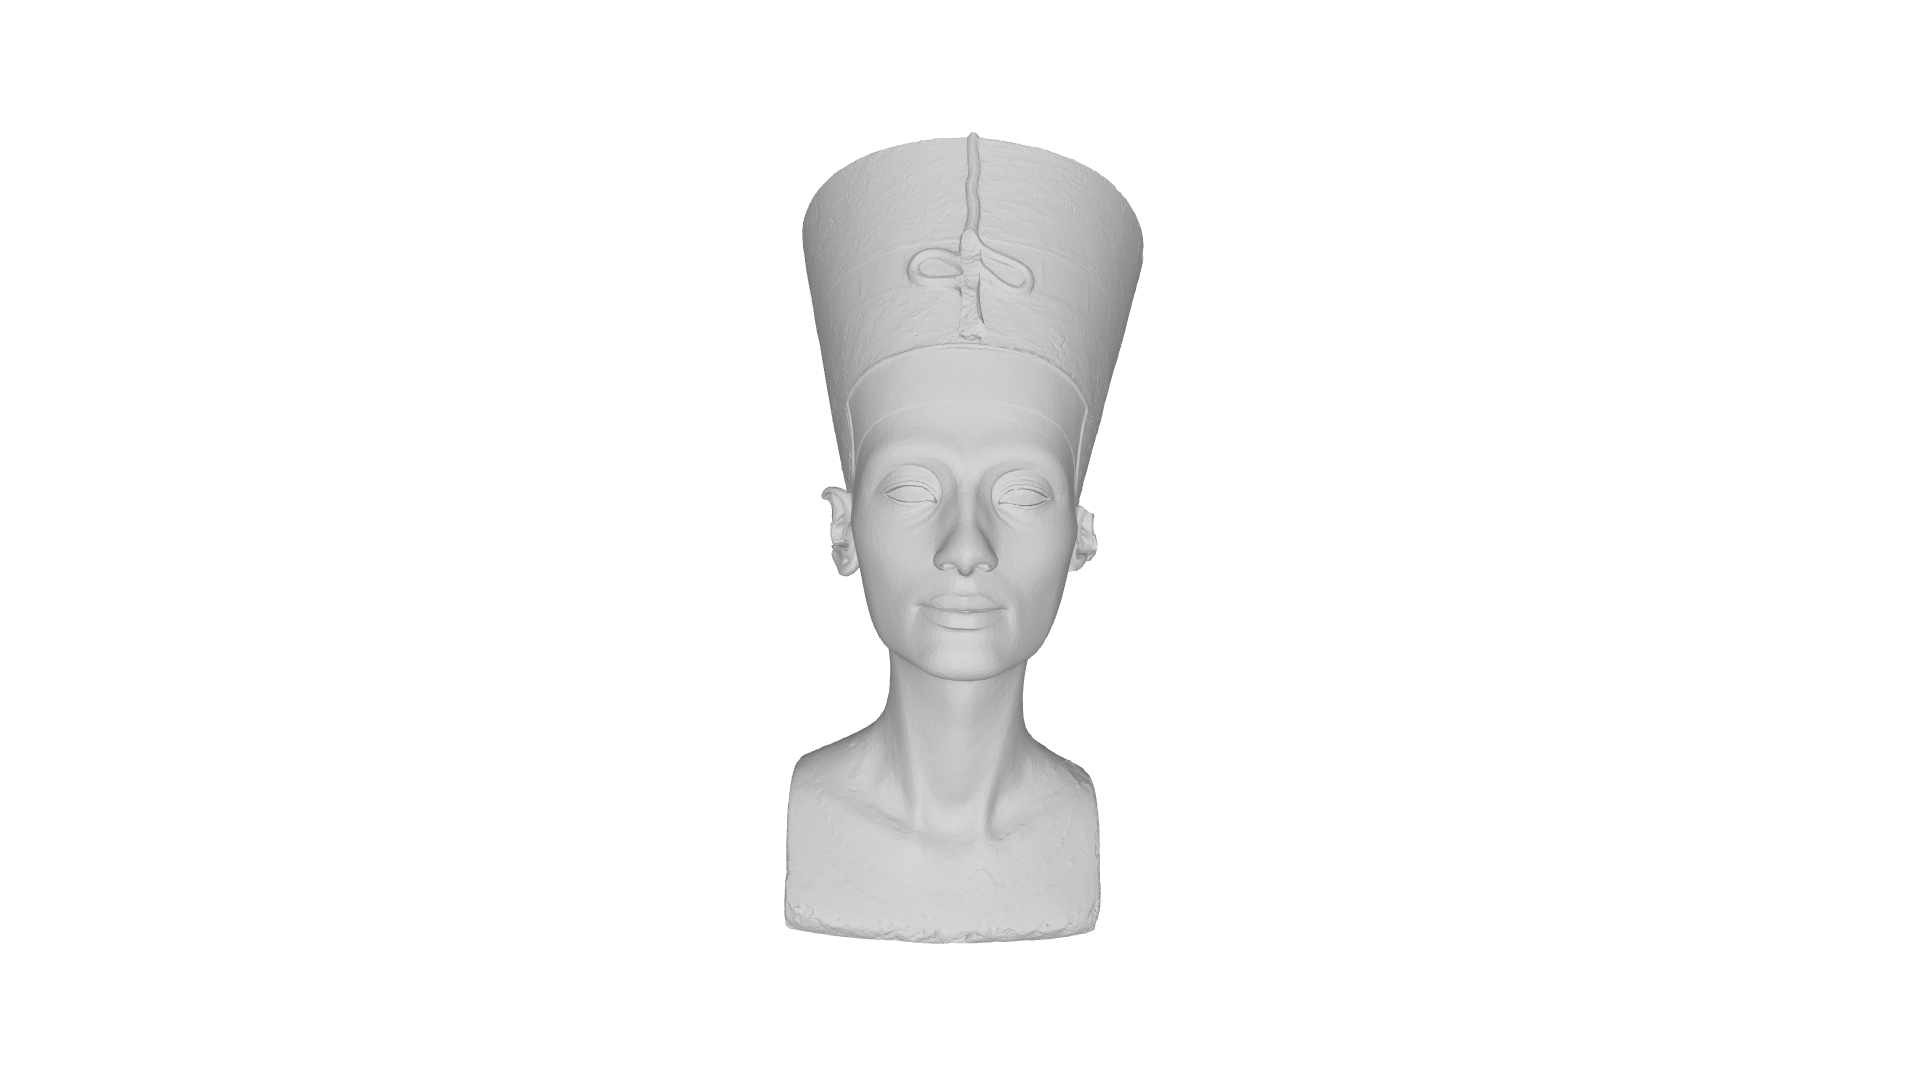
\includegraphics[width=\textwidth]{Figures/results/nefertiti_ground_truth.png}
\caption{Ground Truth}
\label{fig:gt}
\end{subfigure}
\hfill
\begin{subfigure}[b]{0.48\textwidth}
\centering
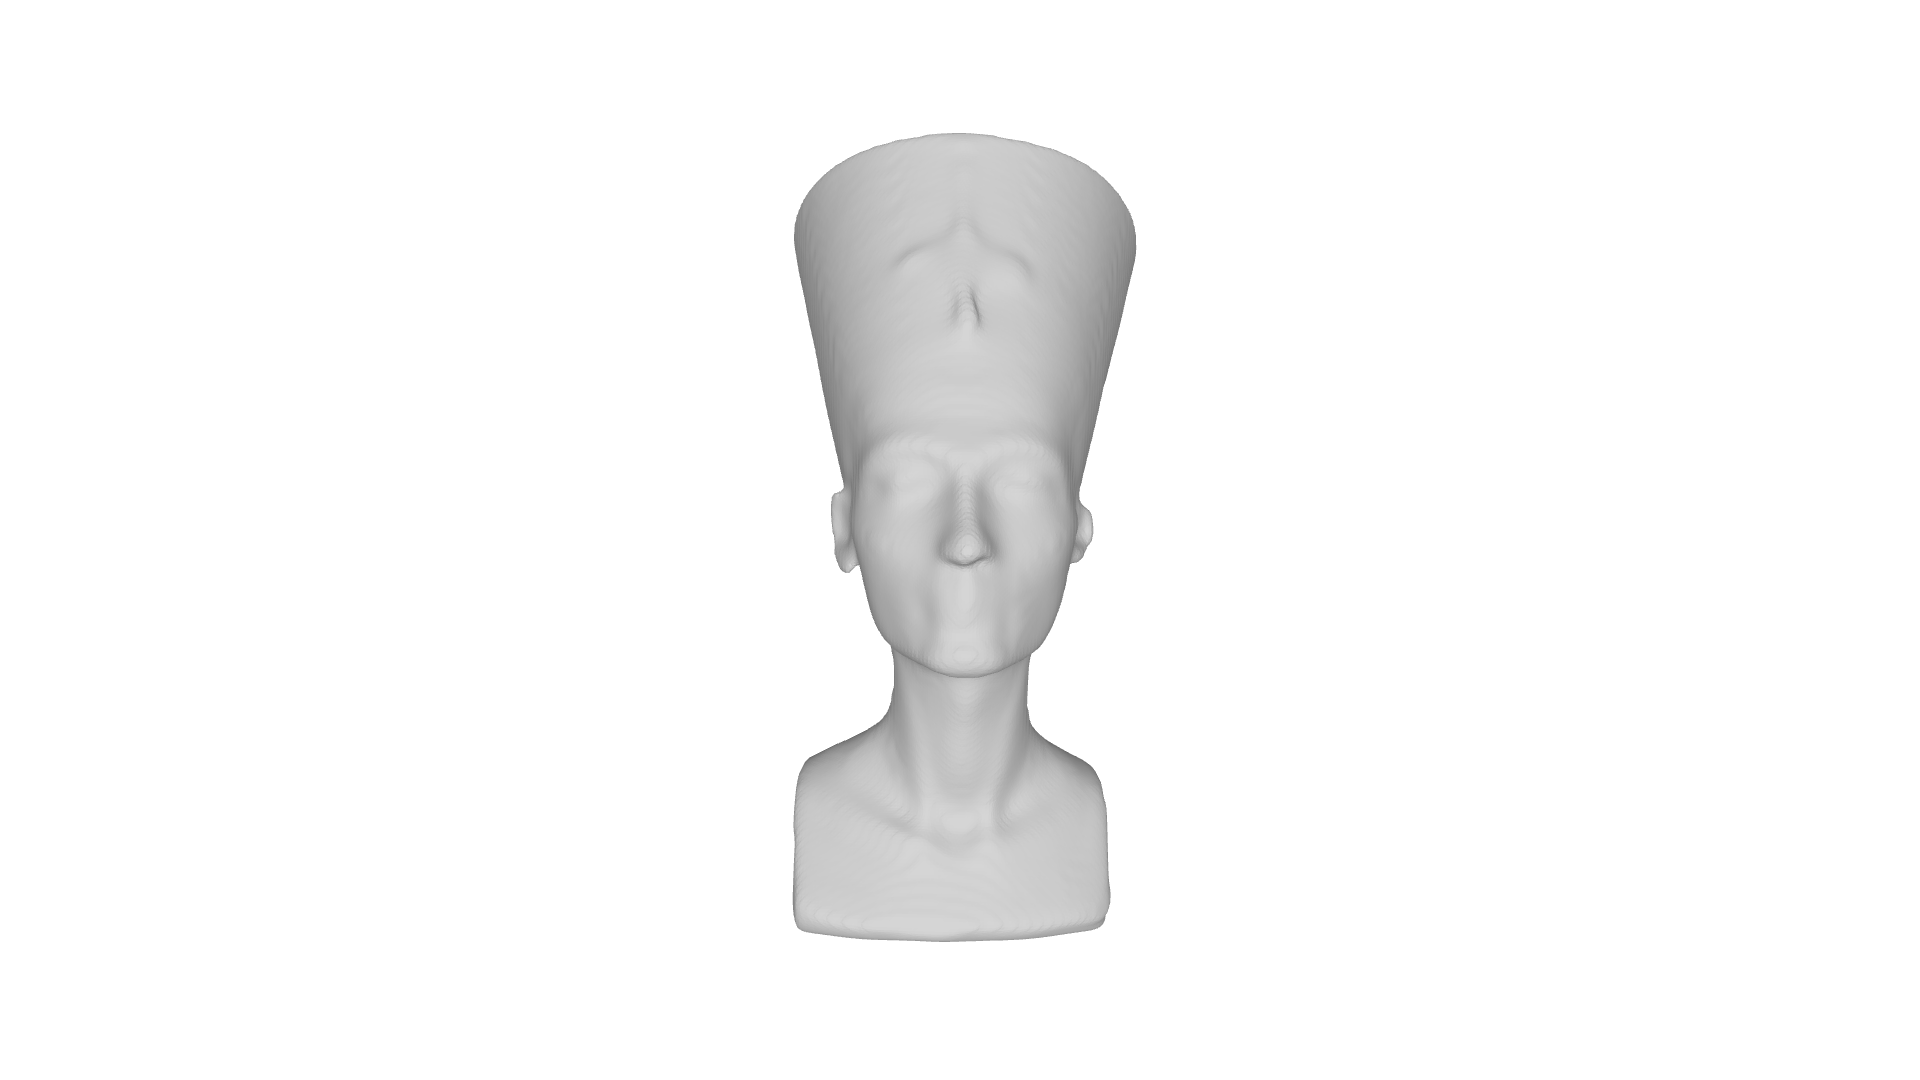
\includegraphics[width=\textwidth]{Figures/results/nefertiti_incode.png}
\caption{INCODE (IoU: 0.9641)}
\label{fig:incode}
\end{subfigure}

\vspace{0.3cm}

\begin{subfigure}[b]{0.48\textwidth}
\centering
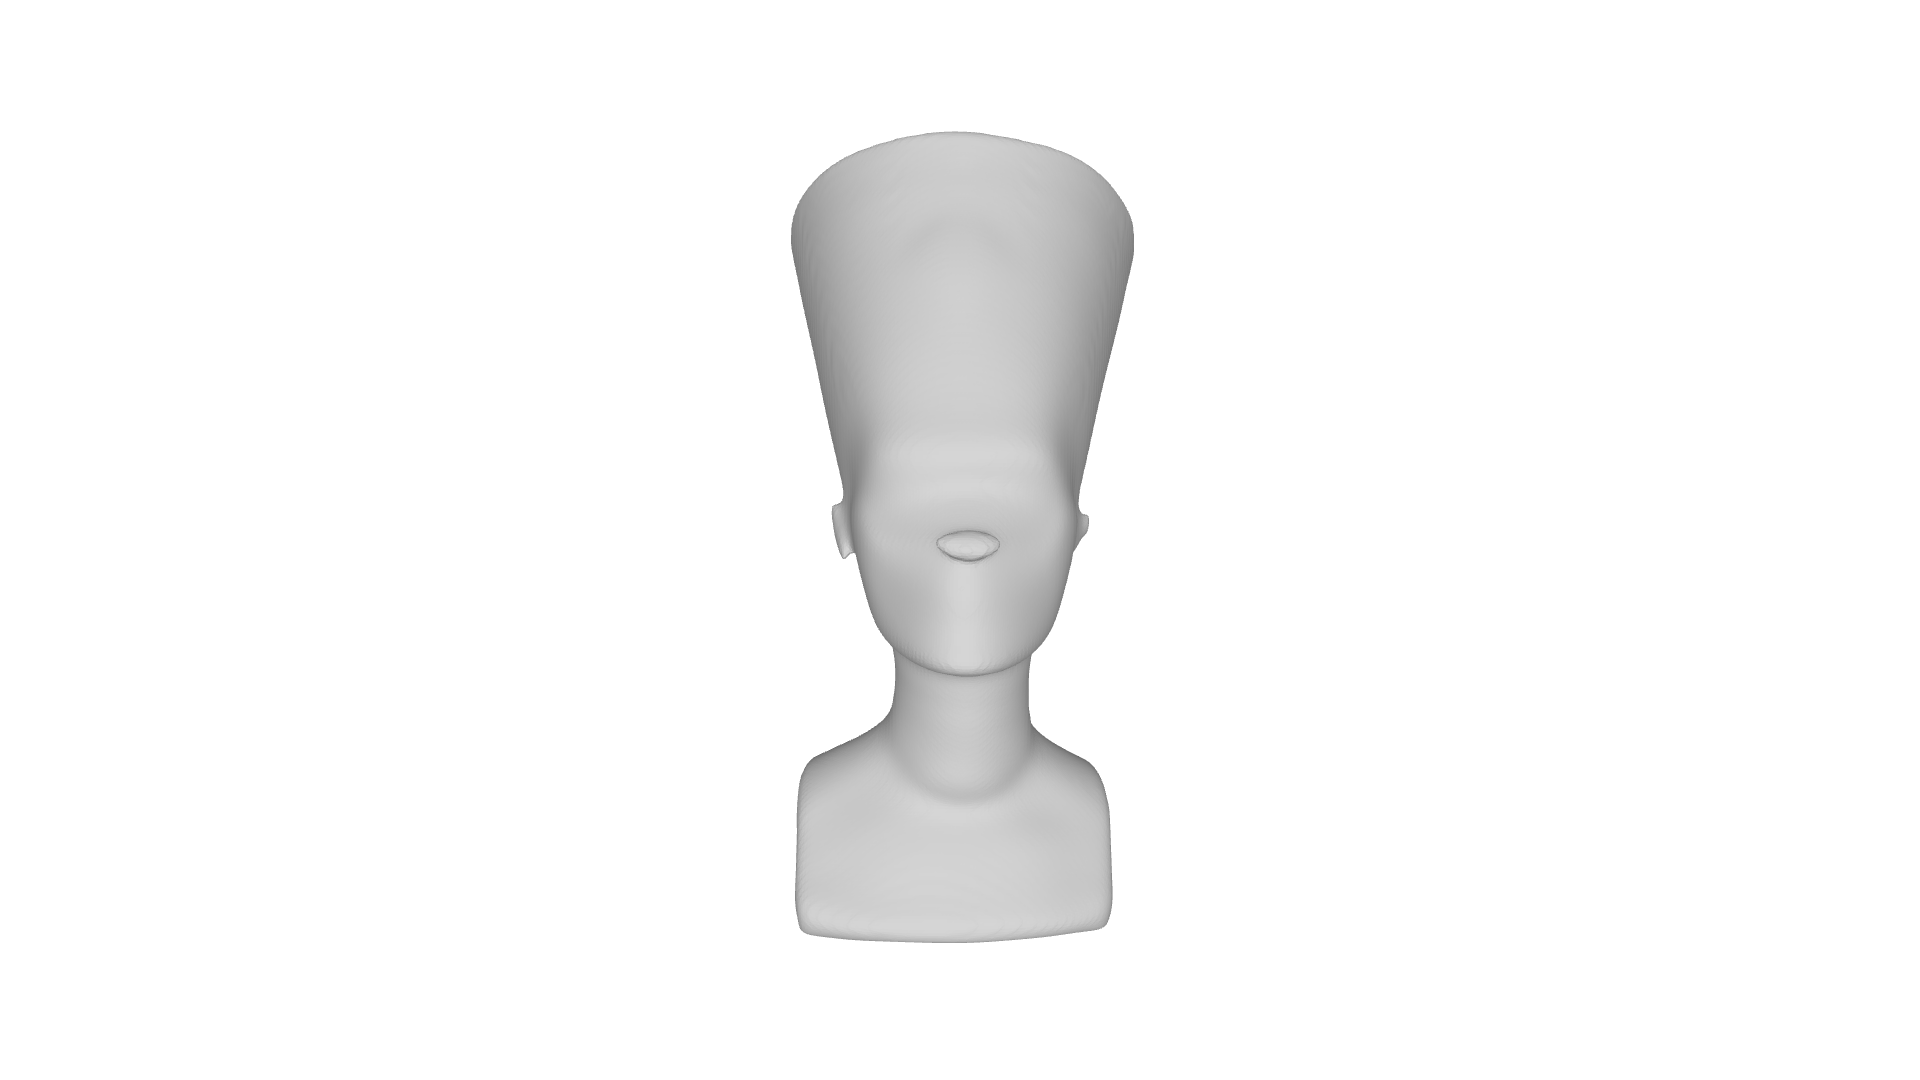
\includegraphics[width=\textwidth]{Figures/results/nefertiti_gauss.png}
\caption{GAUSS (IoU: 0.9158)}
\label{fig:gauss}
\end{subfigure}
\caption{Visual comparison of 3D occupancy reconstruction on the Nefertiti bust. INCODE recovers the silhouette and gross facial structure but loses the headdress band and most of the crown ornament. GAUSS smooths the face away almost entirely. All renders use identical camera position, lighting, and resolution ($1920 \times 1080$).}
\label{fig:reconstruction_comparison}
\end{figure}

The renders temper the quantitative picture considerably. An evaluation IoU above 0.95 sounds close to perfect, but IoU is dominated by the object's interior volume, which every method recovers easily; the surface detail that distinguishes a good reconstruction contributes very little to the score.

INCODE (Fig.~\ref{fig:incode}) recovers the silhouette, crown, neck, and shoulders faithfully, and the nose and brow ridge remain identifiable. Beyond that, detail is lost: the eyes become shallow depressions rather than defined lids, the lips are indistinct, the headdress band has disappeared, and the uraeus ornament survives only as a faint ridge. This is the \emph{best} reconstruction we obtained, and it does not preserve the fine ornamental detail that motivated the choice of this mesh. GAUSS (Fig.~\ref{fig:gauss}) is oversmoothing in its clearest form, consistent with a network that never fit the training data closely: the eyes are absent entirely and the crown is a featureless blob.

All methods lose the crown ornamentation and the headdress edge, differing mainly in how much facial structure survives. At this network size and training budget, none of the eight architectures resolves the detail this mesh was chosen to test.

Figure~\ref{fig:all_methods} presents reconstructions from all eight methods in a two-row grid, ordered by evaluation IoU.

\begin{figure}[htbp]
\centering
% Row 1: Top 4 methods
\begin{subfigure}[b]{0.24\textwidth}
\centering
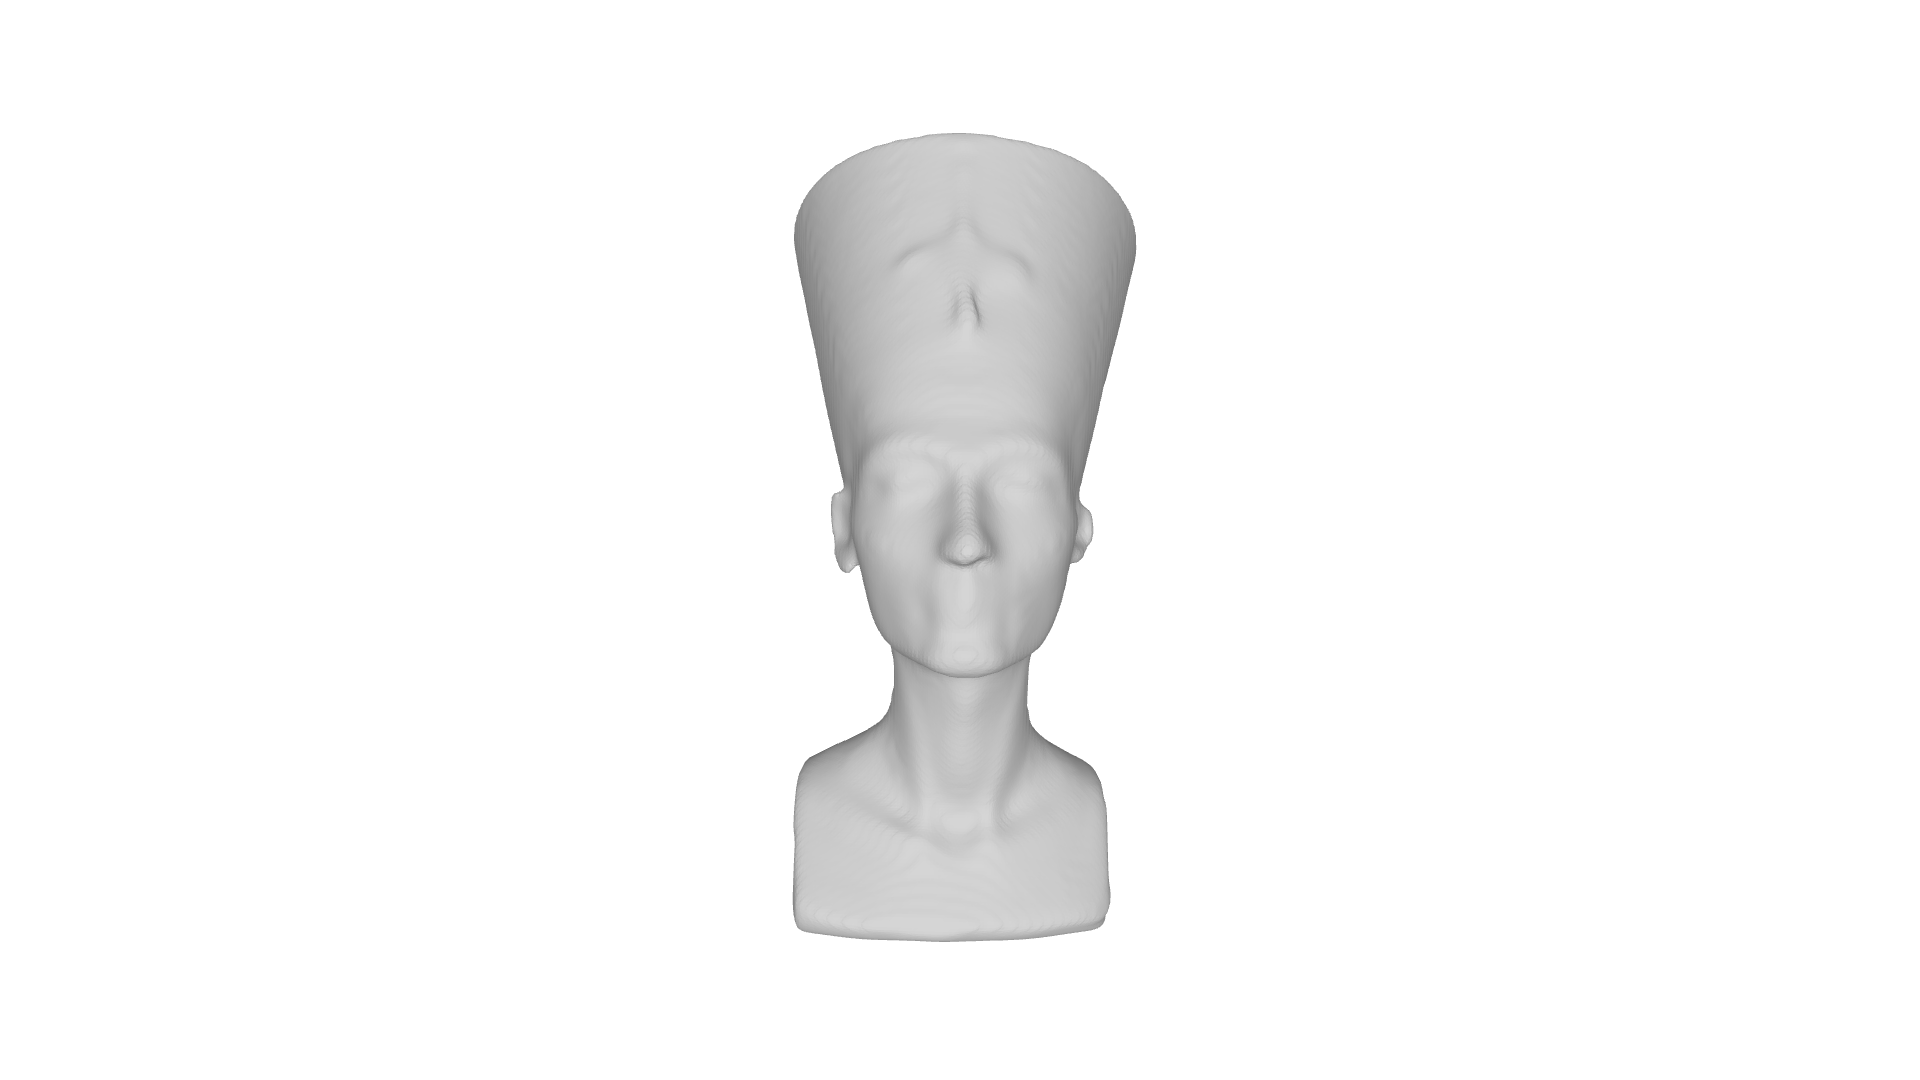
\includegraphics[width=\textwidth]{Figures/results/nefertiti_incode.png}
\caption{INCODE (0.9641)}
\end{subfigure}
\hfill
\begin{subfigure}[b]{0.24\textwidth}
\centering
% NOTE: requires the sigma=1.0 render. Re-render outputs_3d/fourier_nefertiti.obj
% from the corrected run; the sigma=10 image is kept as nefertiti_fourier_sigma10.png.

\includegraphics[width=\textwidth]{Figures/results/nefertiti_fourier.png}
\caption{Fourier (0.9632)}
\end{subfigure}
\hfill
\begin{subfigure}[b]{0.24\textwidth}
\centering
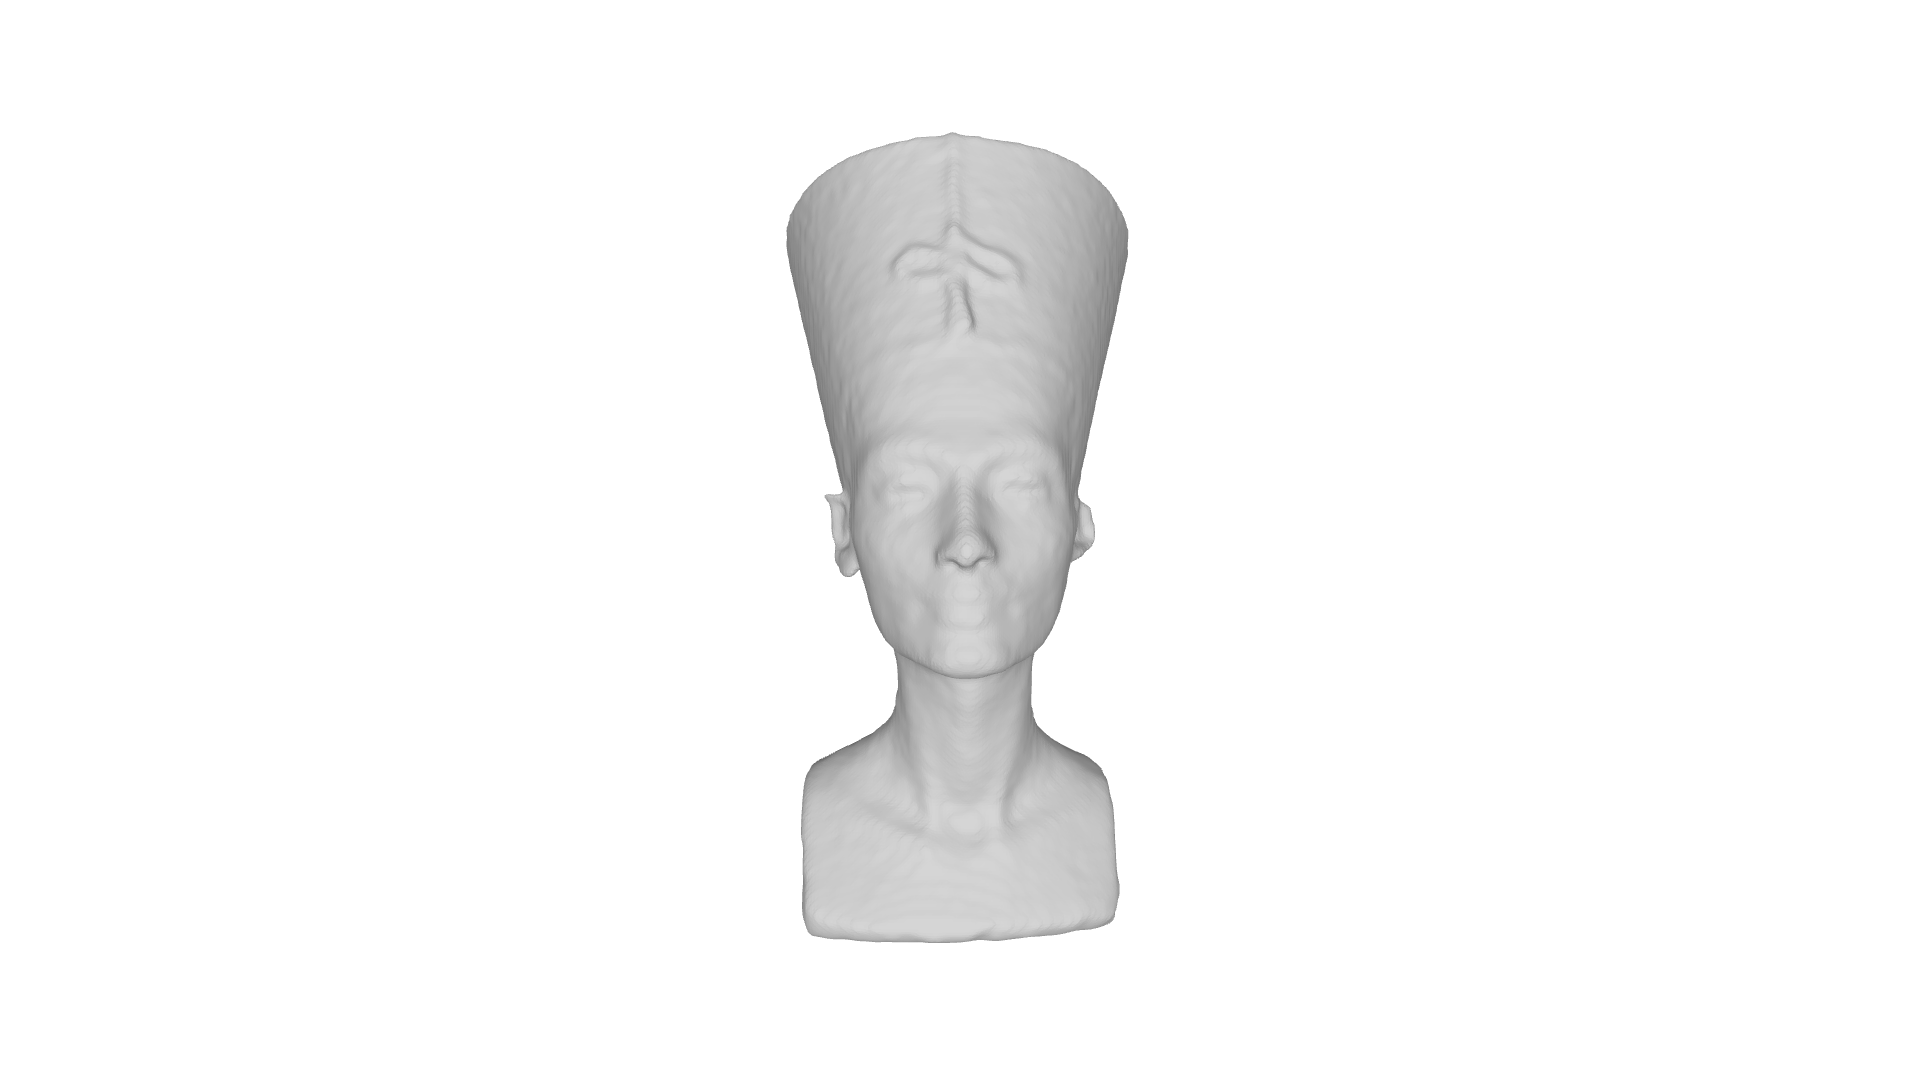
\includegraphics[width=\textwidth]{Figures/results/nefertiti_fr.png}
\caption{FR (0.9606)}
\end{subfigure}
\hfill
\begin{subfigure}[b]{0.24\textwidth}
\centering
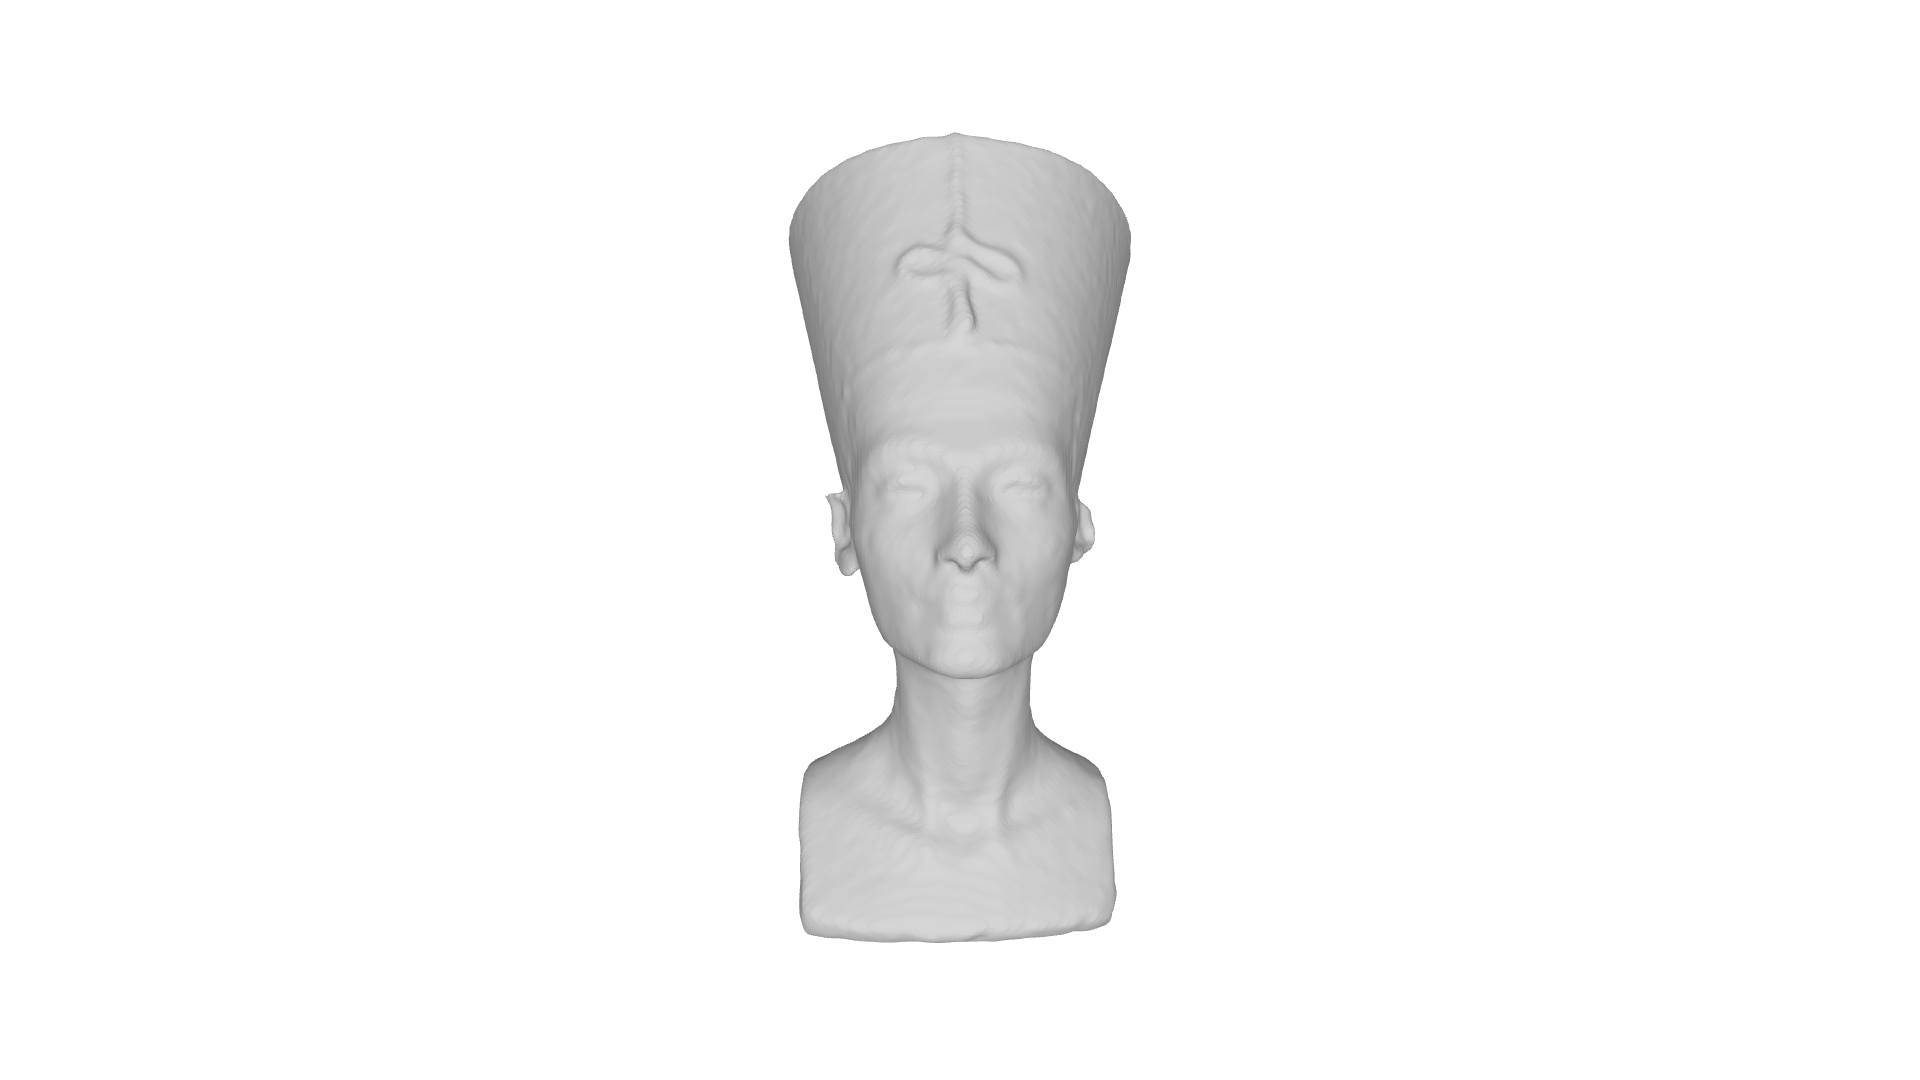
\includegraphics[width=\textwidth]{Figures/results/nefertiti_siren.png}
\caption{SIREN (0.9564)}
\end{subfigure}

\vspace{0.2cm}

% Row 2: remaining methods
\begin{subfigure}[b]{0.24\textwidth}
\centering
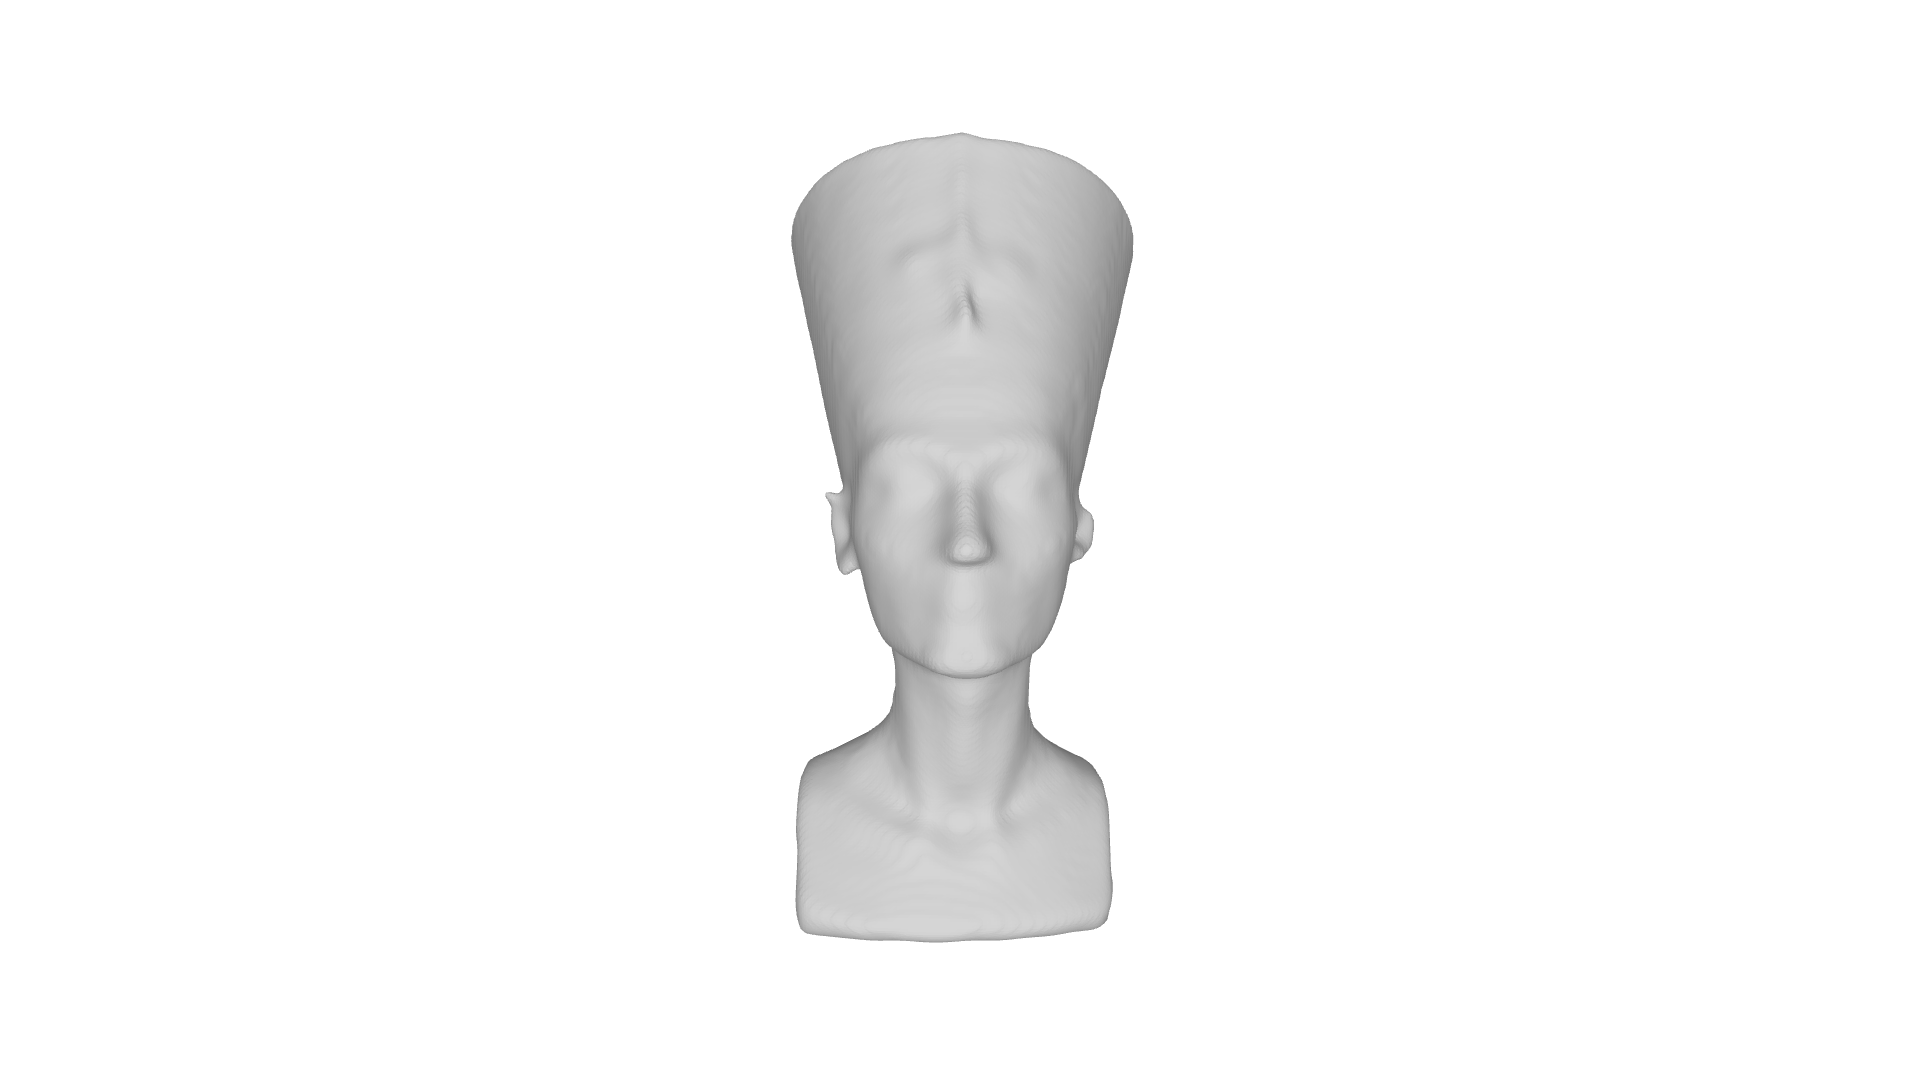
\includegraphics[width=\textwidth]{Figures/results/nefertiti_finer.png}
\caption{FINER (0.9541)}
\end{subfigure}
\hfill
\begin{subfigure}[b]{0.24\textwidth}
\centering
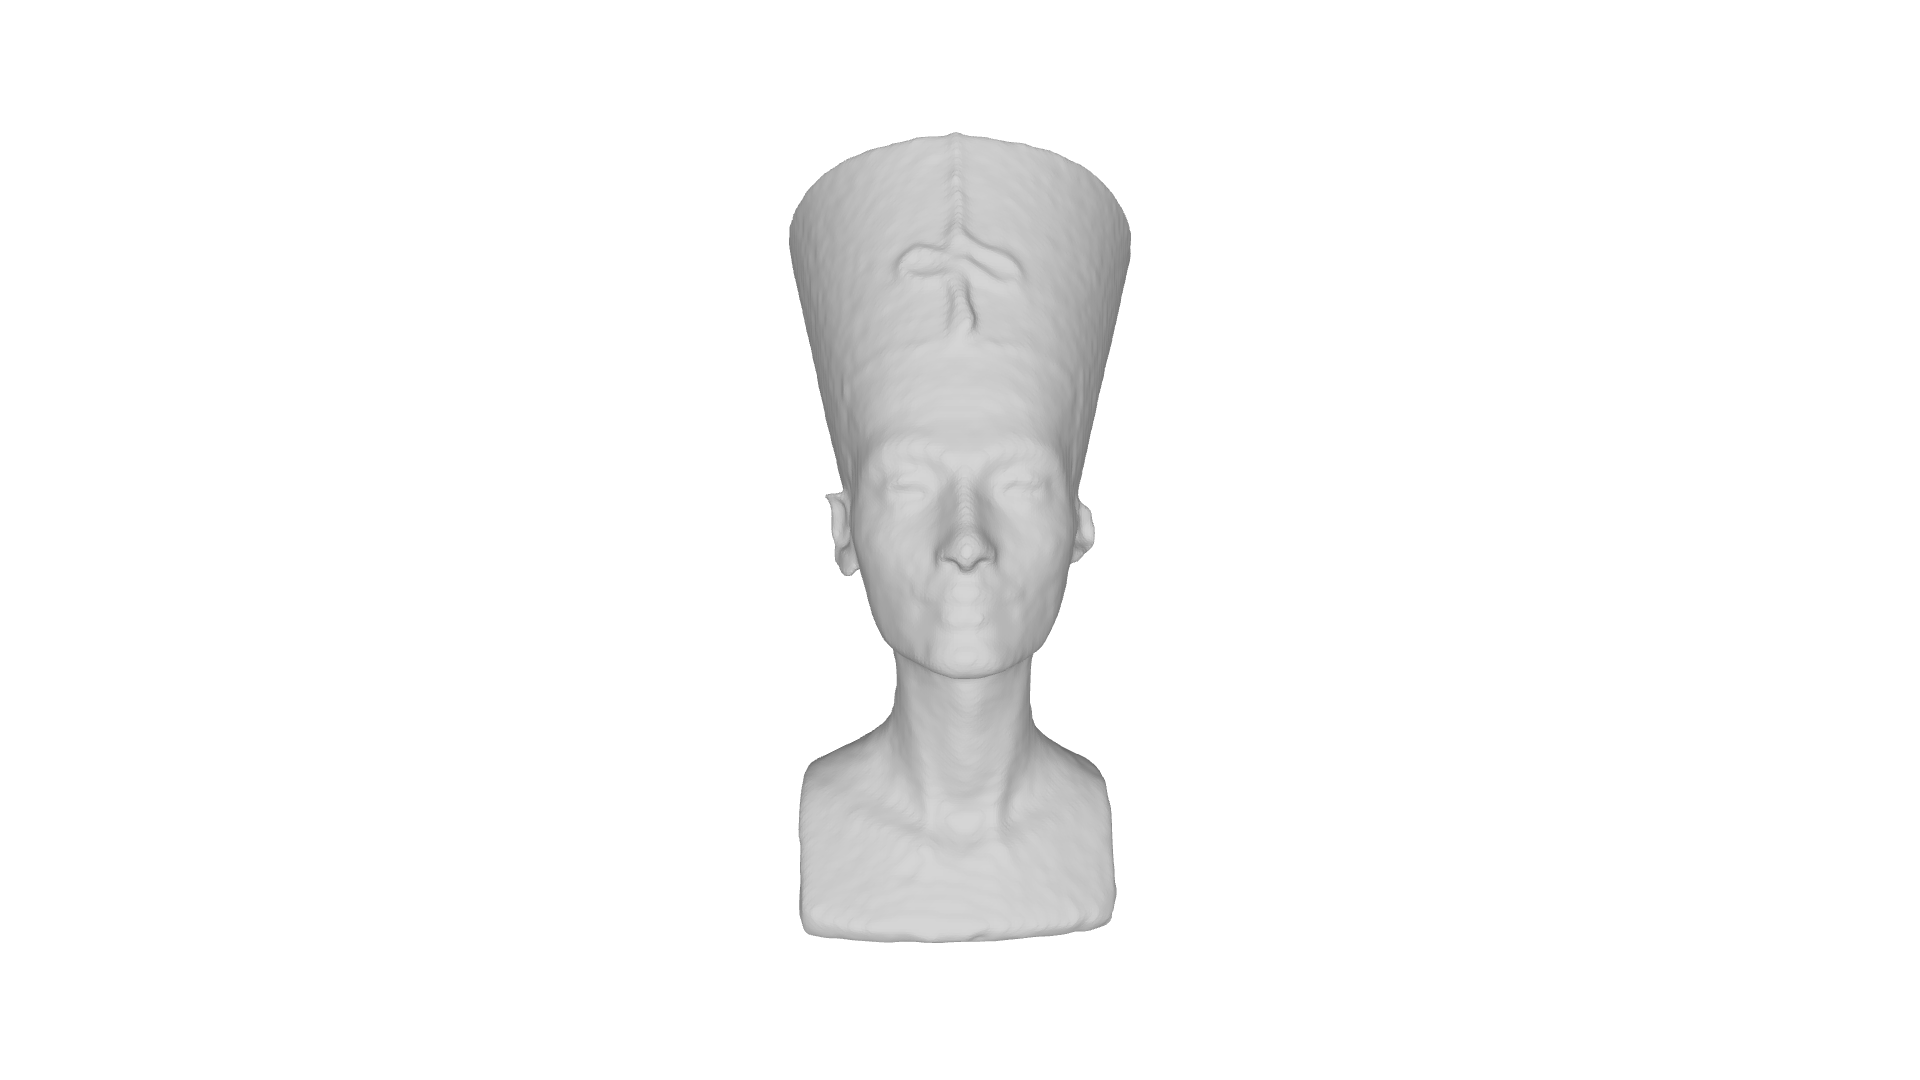
\includegraphics[width=\textwidth]{Figures/results/nefertiti_wire.png}
\caption{WIRE (0.9521)}
\end{subfigure}
\hfill
\begin{subfigure}[b]{0.24\textwidth}
\centering
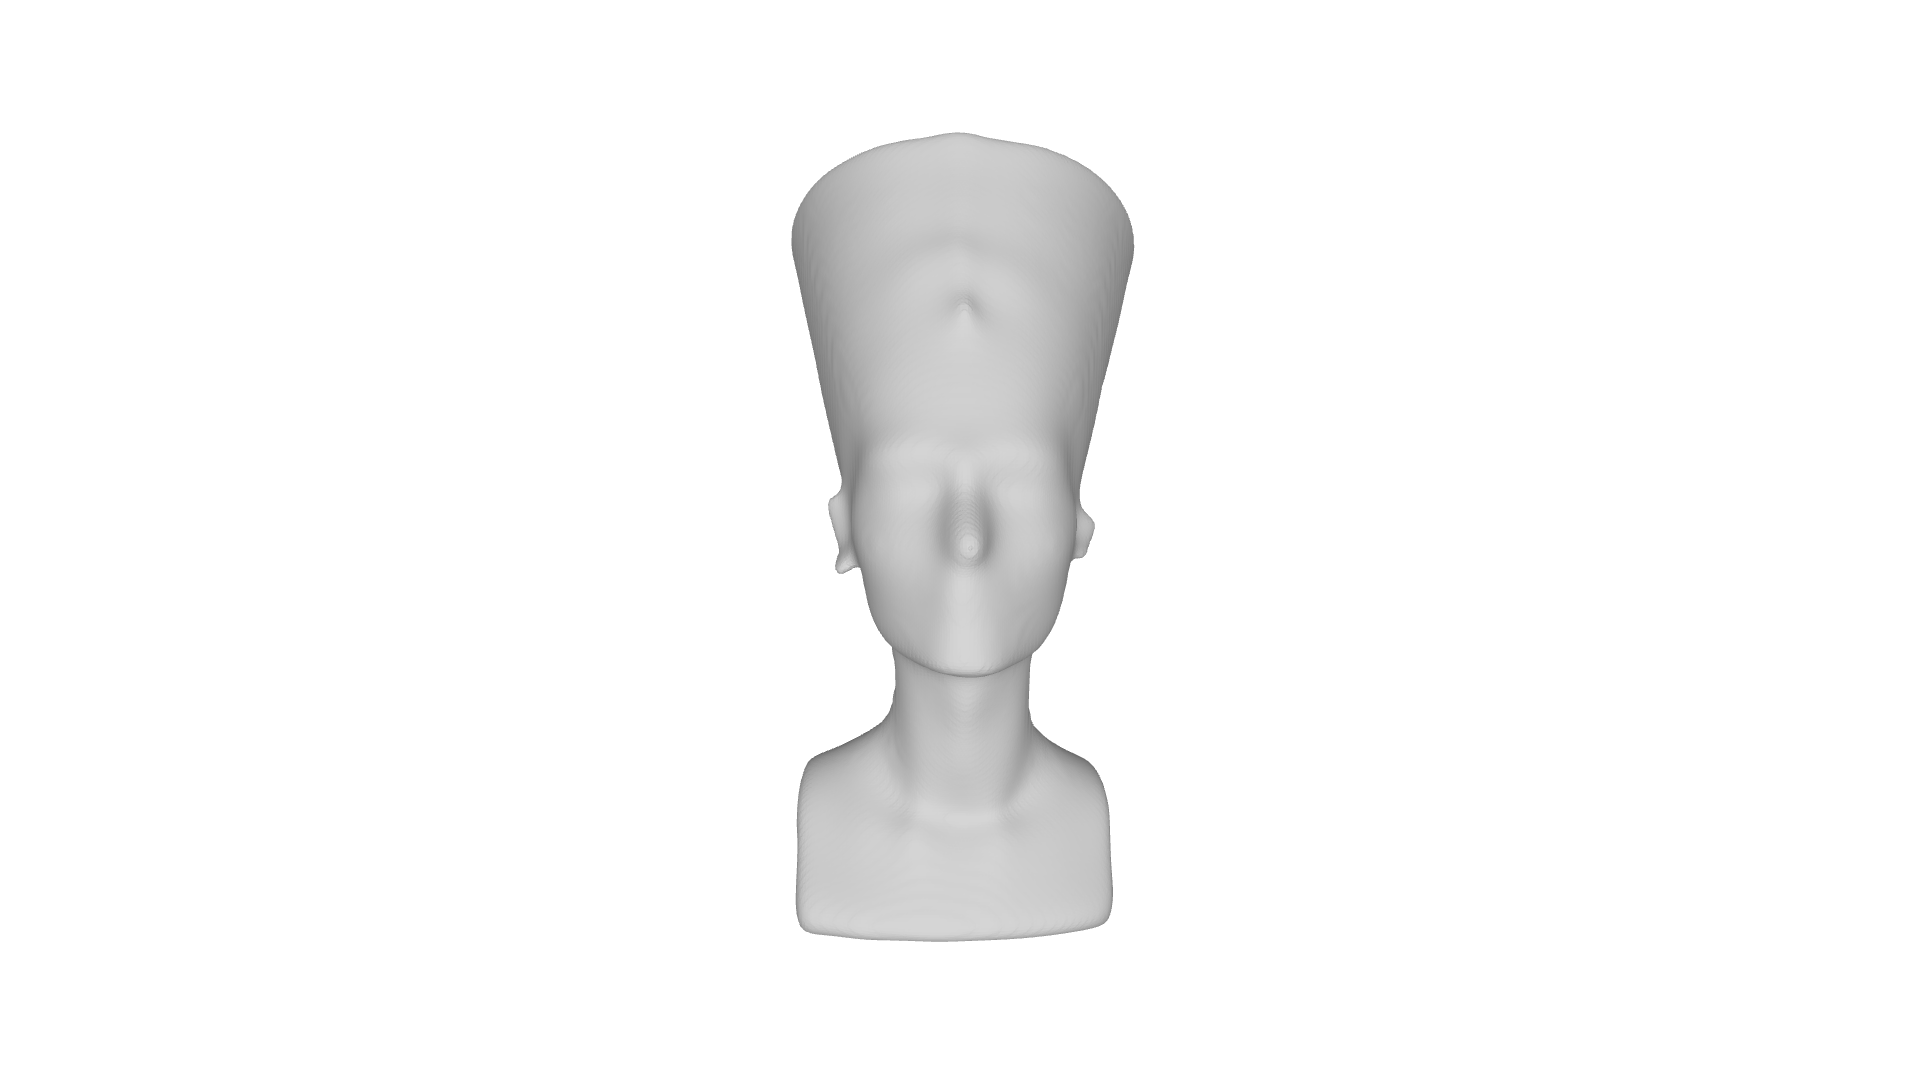
\includegraphics[width=\textwidth]{Figures/results/nefertiti_mfn.png}
\caption{MFN (0.9325)}
\end{subfigure}
\hfill
\begin{subfigure}[b]{0.24\textwidth}
\centering
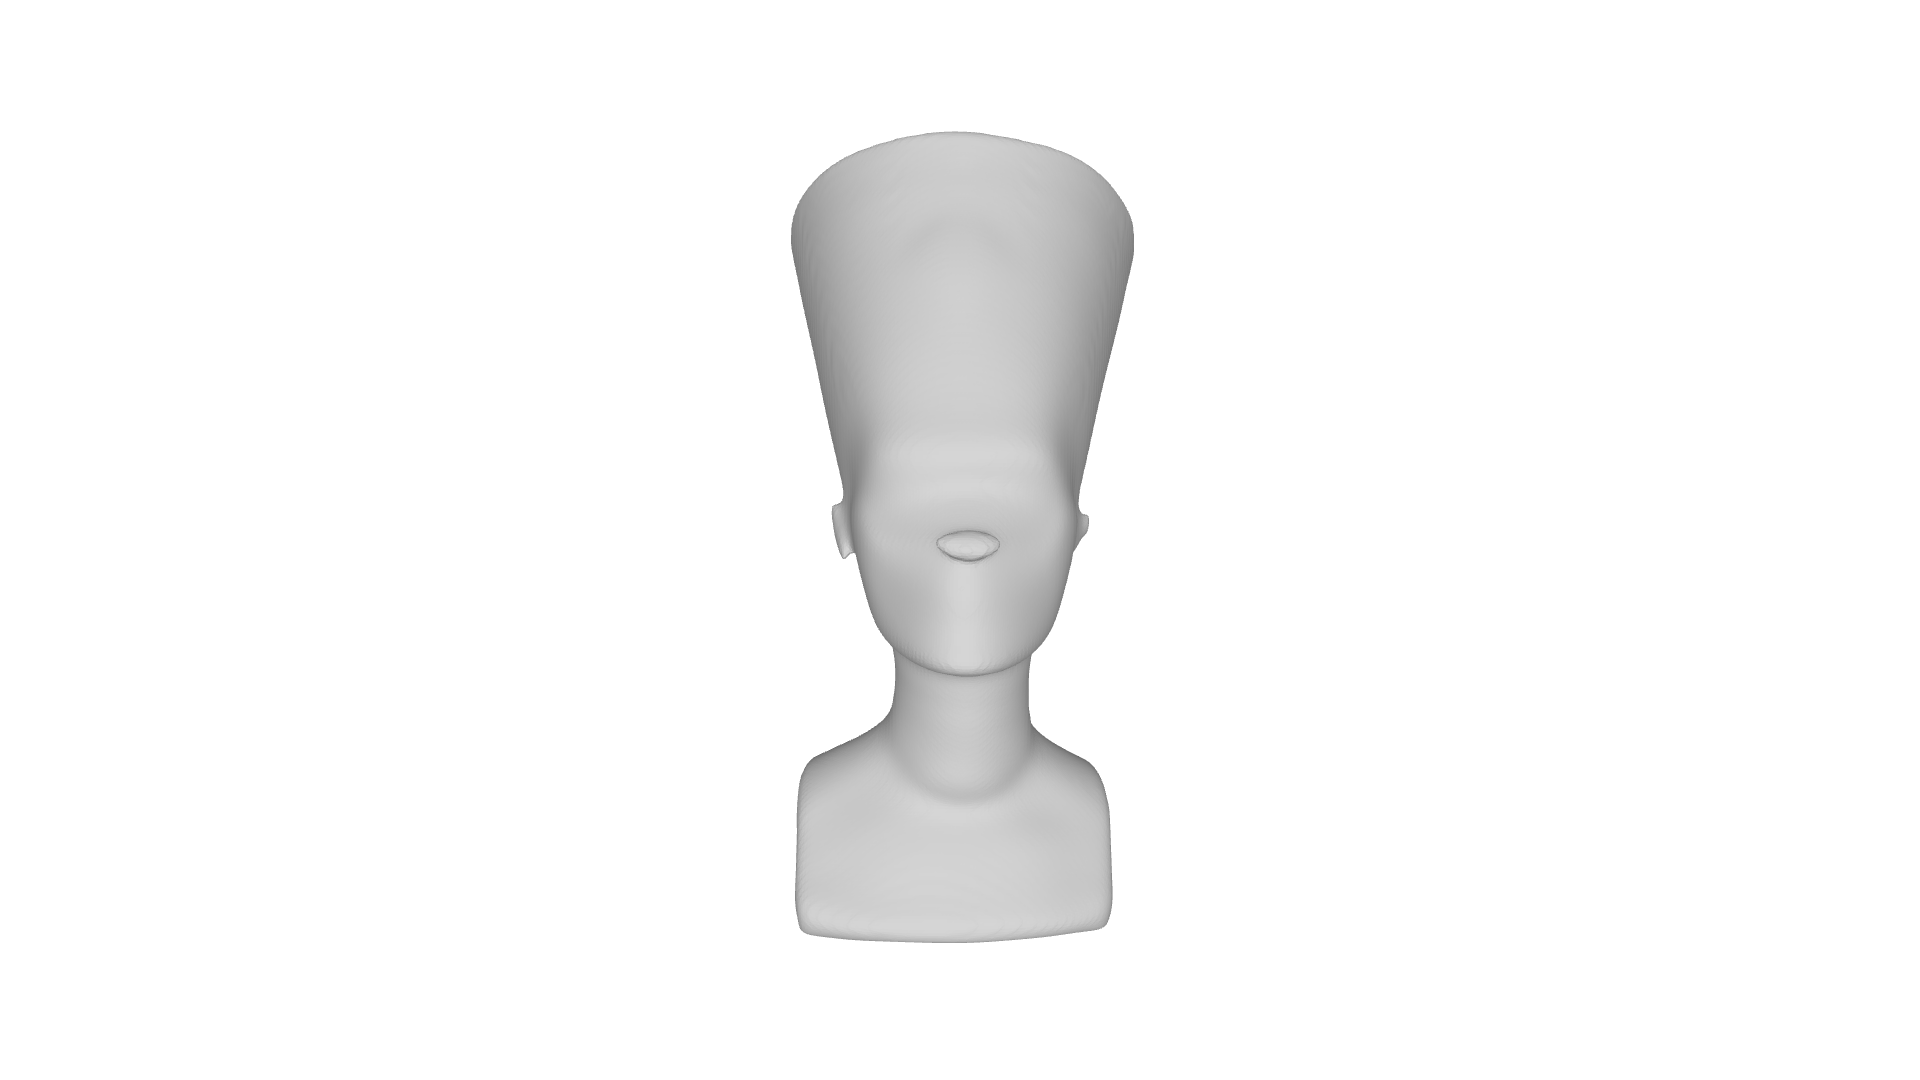
\includegraphics[width=\textwidth]{Figures/results/nefertiti_gauss.png}
\caption{GAUSS (0.9158)}
\end{subfigure}
\caption{Complete visual comparison of all eight INR methods on the Nefertiti bust, ordered by evaluation IoU. Methods are rendered from the same viewpoint with consistent lighting and resolution ($1920 \times 1080$). The six leading reconstructions are difficult to tell apart by eye, consistent with the narrow numerical spread between them; the visible differences appear only in the trailing pair.}
\label{fig:all_methods}
\end{figure}

Two observations follow from the grid. First, the six leading reconstructions are hard to distinguish visually, which is what a 1.2-point IoU spread across a single run of each method should look like. We would not be able to identify the ranking from these images alone, and we do not claim the numerical ordering is meaningful. Second, the visible differences are confined to the trailing pair: MFN and GAUSS visibly smooth the geometry away, and both fall outside the leading cluster numerically as well.

\section{Analysis by Architectural Properties}
\label{sec:properties}

\subsection{Frequency Compactness Does Not Survive a Sensitivity Check}

Following the taxonomy in Chapter~\ref{ch:background}, we group methods by whether they possess frequency compactness (FINER, INCODE, GAUSS, WIRE) or not (SIREN, Fourier Features, FR, MFN) and compare group means.

On the corrected results, the frequency-compact group averages 0.9465 against 0.9532 for the others: a 0.67 percentage point advantage for methods \emph{lacking} frequency compactness. Taken alone, this would be reported as weak evidence against the property mattering for 3D occupancy.

That reading is not stable, and two perturbations show why. First, our earlier Fourier Features run differed from the reported one in a single hyperparameter, the frequency scale $\sigma$. With $\sigma = 10.0$ instead of $1.0$, Fourier Features falls to 0.7966 and drags its group's mean down to 0.9115, at which point frequency compactness appears to confer a decisive 3.5 point \emph{advantage}. One hyperparameter of one method, leaving the other seven untouched, reverses the sign of the conclusion and changes its magnitude five-fold.

Second, the result is equally sensitive to which methods are included. Dropping GAUSS --- the weakest run, and a frequency-compact one --- raises that group's mean to 0.9568 and restores a 0.36 point advantage for frequency compactness, again reversing the sign.

A grouped mean over four methods, each run once, is therefore not a sound basis for ranking architectural properties. The conclusion flips under two independent perturbations, each individually defensible, and nothing in the analysis itself signals this instability. We report it as a negative methodological result: establishing whether frequency compactness matters for 3D occupancy would require several seeds per method, a variance estimate, and a significance test, none of which this experiment provides.

\subsection{Interaction with Adaptivity}

The same caution applies to adaptivity, though the comparison is less fragile because it does not involve the failed run. Among frequency-compact methods, those with adaptivity (FINER, INCODE) average 0.9591 against 0.9339 for the non-adaptive pair (GAUSS, WIRE), a gap of 2.5 percentage points. This is consistent with adaptive frequency allocation being useful, but with two methods per group and one run each, it remains suggestive rather than demonstrated.

Adaptivity alone certainly does not determine the outcome. FR possesses adaptivity but lacks frequency compactness, and places second overall; GAUSS lacks adaptivity and places last among valid runs. Both observations are compatible with a wide range of explanations, including the eight-fold difference in parameter counts across methods discussed in Section~\ref{sec:setup}.

\section{Computational Efficiency}

Training cost is remarkably uniform. Seven of the eight methods complete 500 epochs within a 10\% band, from 2635 seconds (SIREN) to 2896 seconds (MFN). Only WIRE stands apart at 3927 seconds, roughly 49\% slower than the fastest, for the reasons given in Section~\ref{ch:implementation}.

For this workload, then, training time is not a meaningful basis for choosing between methods, with the single exception of avoiding WIRE when compute is constrained. Dividing quality by time reflects this: SIREN attains the best ratio at 0.0218 IoU per minute simply by being fastest. We report the ratio in Table~\ref{tab:training_time} for completeness but attach little weight to it, since the numerator differences are within run-to-run noise.

\section{Training Dynamics}

The gap between final training IoU and evaluation IoU separates the methods into two clear regimes, and this split is more informative than the ranking itself.

Three methods fit the training data essentially perfectly and lose ground at evaluation: SIREN and WIRE both reach a training IoU of 1.0000 while evaluating at 0.9564 and 0.9521, and FR reaches 0.9976 while evaluating at 0.9606. Gaps of 3.7 to 4.8 points indicate these networks are partly memorizing point labels. This is a direct consequence of the fixed dataset described in Chapter~\ref{ch:methodology}: because the same 450,000 points are revisited every epoch, nothing prevents a sufficiently expressive network from fitting them individually.

Two methods show the opposite behaviour. MFN reaches a training IoU of only 0.9385 and GAUSS only 0.9126 --- in the latter case, \emph{below} its evaluation IoU of 0.9158. These methods are not oversmoothing at evaluation time; they never fit the training data in the first place. Their weakness is an optimization failure, which is consistent with both requiring learning-rate overrides to converge at all.

INCODE and FINER sit between these regimes, with gaps under one point (0.9725/0.9641 and 0.9628/0.9541). They neither memorize nor underfit, which is the most plausible explanation for INCODE placing first. Fourier Features is intermediate, with a gap of 2.6 points (0.9892/0.9632) --- larger than INCODE's but well short of the memorizing group.

The regimes correspond only loosely to final performance. WIRE memorizes and places sixth; FR memorizes and places third. The train--eval gap explains \emph{how} a method fails when it does, but it does not by itself order the leading group.

\section{Failure Mode Characterization}

\subsection{GAUSS and MFN: Optimization Failure, Not Oversmoothing}

It would be natural to attribute GAUSS's oversmoothed reconstruction (Fig.~\ref{fig:gauss}) to the limited frequency coverage of its rapidly decaying activation, and MFN's weakness to its multiplicative composition. The training IoUs reported above rule this out: a network that cannot fit data it has already seen has not shown that it \emph{could not} represent the target function, only that this optimizer at this learning rate did not find the parameters. Separating the two would require a learning-rate sweep per method, which our fixed protocol excluded --- an exclusion that disadvantages precisely the methods most sensitive to it.

\subsection{Frequency Scale: A Single-Parameter Ablation}
\label{sec:fourier_ablation}

The Fourier Features encoding is governed by two separate parameters: the number of random frequencies $m$, which sets the width of the encoded input, and the scale $\sigma$, which controls how high those frequencies reach. Only $\sigma$ affects frequency content. Because we ran this architecture at both $\sigma = 1.0$ and $\sigma = 10.0$ with everything else held fixed, the pair forms a controlled ablation on frequency scale --- the only such comparison in our results, and the largest effect we measured from any single hyperparameter.

\begin{table}[htbp]
\centering
\caption{Effect of the frequency scale $\sigma$ on Fourier Features, with all other settings held fixed ($m = 256$, 4 hidden layers, 500 epochs).}
\label{tab:sigma_ablation}
\begin{tabular}{lccccc}
\toprule
$\sigma$ & \textbf{Train IoU} & \textbf{Eval IoU} & \textbf{Gap} & \textbf{Chamfer-L1} & \textbf{Normal Cons.} \\
\midrule
1.0  & 0.9892 & \textbf{0.9632} & 0.0260 & \textbf{0.010973} & \textbf{0.9809} \\
10.0 & 1.0000 & 0.7966 & 0.2034 & 0.051407 & 0.6542 \\
\bottomrule
\end{tabular}
\end{table}

\begin{figure}[htbp]
\centering
\begin{subfigure}[b]{0.48\textwidth}
\centering
% NOTE: requires the sigma=1.0 render (see Fig. 5.2 note).

\includegraphics[width=\textwidth]{Figures/results/nefertiti_fourier.png}
\caption{$\sigma = 1.0$ (Eval IoU: 0.9632)}
\label{fig:fourier_s1}
\end{subfigure}
\hfill
\begin{subfigure}[b]{0.48\textwidth}
\centering
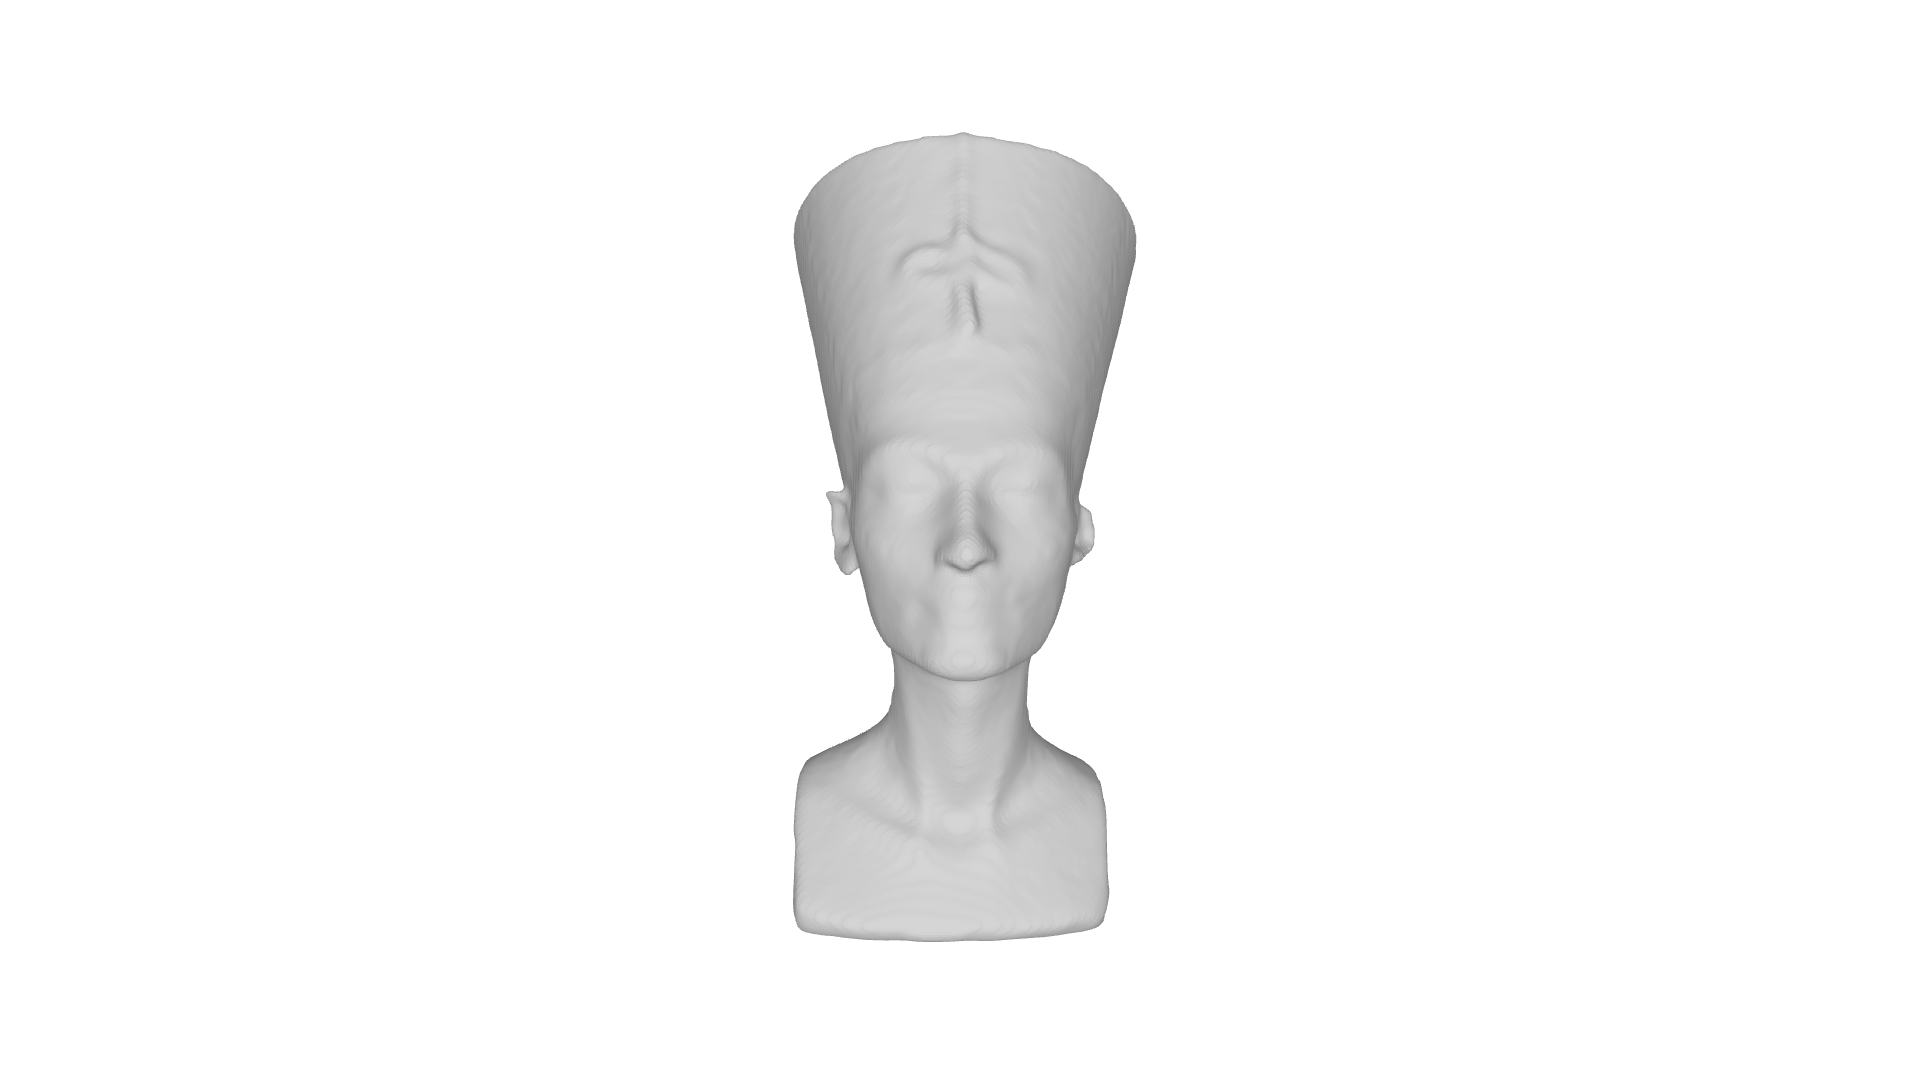
\includegraphics[width=\textwidth]{Figures/results/nefertiti_fourier_sigma10.png}
\caption{$\sigma = 10.0$ (Eval IoU: 0.7966)}
\label{fig:fourier_s10}
\end{subfigure}
\caption{Effect of the frequency scale $\sigma$ on Fourier Features, with all other settings identical. At $\sigma = 10.0$ the reconstruction is distorted rather than smoothed: the face is melted and asymmetric, the eye sockets are hollowed out, the mouth is lost, and wave-like ripples run across the crown and shoulders. These ripples are the signature of an encoding oscillating between correctly classified training points. The same architecture at $\sigma = 1.0$ is competitive with the best method tested.}
\label{fig:sigma_ablation}
\end{figure}

Raising $\sigma$ by one order of magnitude costs 16.7 points of evaluation IoU while \emph{improving} training IoU to a perfect 1.0000. Chamfer-L1 degrades by a factor of nearly five and normal consistency collapses from 0.9809 to 0.6542. At $\sigma = 10.0$ the encoding samples frequencies far above anything present in the geometry, and the network reproduces its training points while oscillating between them; at $\sigma = 1.0$ the same architecture is competitive with the best method we tested.

Three things make this worth reporting. The effect dwarfs every difference between architectures in this study: 16.7 points, against the 1.2 points separating the six leading methods. It is entirely invisible in the training signal, which improves as the model gets worse, so any workflow monitoring only training loss would have shipped the failed configuration. And it demonstrates that a conclusion about \emph{architectures} can be dominated by a hyperparameter within one of them --- the mechanism behind the instability documented in Section~\ref{sec:properties}. None of this is evidence against random Fourier features, which are well established~\cite{tancik2020fourier}; it is evidence that the frequency scale must be matched to the target geometry.

\section{Summary of Experimental Findings}

\begin{itemize}
    \item \textbf{Six methods are indistinguishable at this sample size.} INCODE (0.9641), Fourier Features (0.9632), FR (0.9606), SIREN (0.9564), FINER (0.9541), and WIRE (0.9521) span 1.2 percentage points across single runs with unseeded initialization, with the top two separated by 0.0009. We report the ordering but do not claim it is meaningful, and the reconstructions in Fig.~\ref{fig:all_methods} are correspondingly hard to tell apart.

    \item \textbf{Two methods are clearly weaker, for optimization rather than representational reasons.} MFN (0.9325) and GAUSS (0.9158) trail by 3.2 to 4.8 points, but both fail on the training set itself and both needed learning-rate overrides.

    \item \textbf{One hyperparameter outweighs every architectural difference.} Changing the Fourier frequency scale from $\sigma = 1.0$ to $\sigma = 10.0$ costs 16.7 IoU points --- fourteen times the spread separating the six leading architectures --- while improving training IoU to 1.0000.

    \item \textbf{The property analysis is not robust.} Frequency compactness appears to matter ($+3.5$ pp), not to matter ($-0.67$ pp), or to matter slightly ($+0.36$ pp) depending on one method's hyperparameter or on whether the weakest run is included. We treat this as evidence that the grouped-mean methodology is inadequate at this sample size, not as a finding about the property.

    \item \textbf{Compute cost does not discriminate.} Seven methods train within a 10\% band; only WIRE is materially slower, at 49\% above the fastest.

    \item \textbf{No method resolves the fine detail the mesh was chosen to test.} Even the best reconstruction loses the headdress band and most of the crown ornament, a limitation invisible in an IoU score dominated by interior volume.
\end{itemize}
